\section{Methodology}
\label{sec:methodology}

\vspace{-0.5em}
As illustrated in \Cref{fig:framework_overview}, \name first estimates teacher--student policy discrepancy from a student-proposed response using the $k_3$ estimator.
The resulting score determines the probability of retaining the proposal or replacing it with a teacher-regenerated response.
The selected response is executed to update the interaction history and added to the training buffer.
During optimization, an importance ratio corrects the sampling distribution of teacher-generated tokens to account for the generating policy, recovering the conditional reverse-KL expectation for teacher-generated tokens.
\vspace{-0.5em}

\subsection{Problem Formulation}
\label{sec:problem_formulation} 

\vspace{-0.5em}
\paragraph{Multi-Turn Agentic Task.}
Given a query $q\sim\mathcal{D}$, an agent interacts with an environment over multiple turns to solve the task~\citep{YaoZYDSN023,ShridharYCBTH21,WangJCA22}.
At turn $t$, the agent observes $o_t$ and samples a response $a_t\sim\pi_\theta(\cdot\mid h_t)$ from its policy $\pi_\theta$, conditioned on the interaction history $h_t=(q,o_1,a_1,\ldots,o_{t-1},a_{t-1},o_t)$.
Each response contains natural-language reasoning and possible subsequent tool calls, environment actions, and the final answer.
For each tool call or environment action, the environment executes the operation specified in $a_t$ and returns a new observation $o_{t+1}\sim P(\cdot\mid h_t,a_t)$.
This loop continues until termination, yielding a trajectory $\tau=(q,o_1,a_1,\ldots,o_H,a_H)$ of $H$ turns, with terminal feedback omitted.
We denote its distribution by $p_{\pi_\theta}(\tau\mid q)$. 
Within each turn, the response $a_t=(x_{t,1},\ldots,x_{t,L_t})$ is generated autoregressively, where $L_t$ is its length.
Given the token-level context $c_{t,k}=(h_t,x_{t,<k})$, its probability factorizes as
\begin{equation}
    \setlength\abovedisplayskip{1pt}
    \setlength\belowdisplayskip{1pt}
    \pi_\theta(a_t\mid h_t)
    =\prod_{k=1}^{L_t}\pi_\theta(x_{t,k}\mid c_{t,k}).
    \label{eq:turn_policy_factorization}
\end{equation}

\begin{figure}[t]
    \centering
    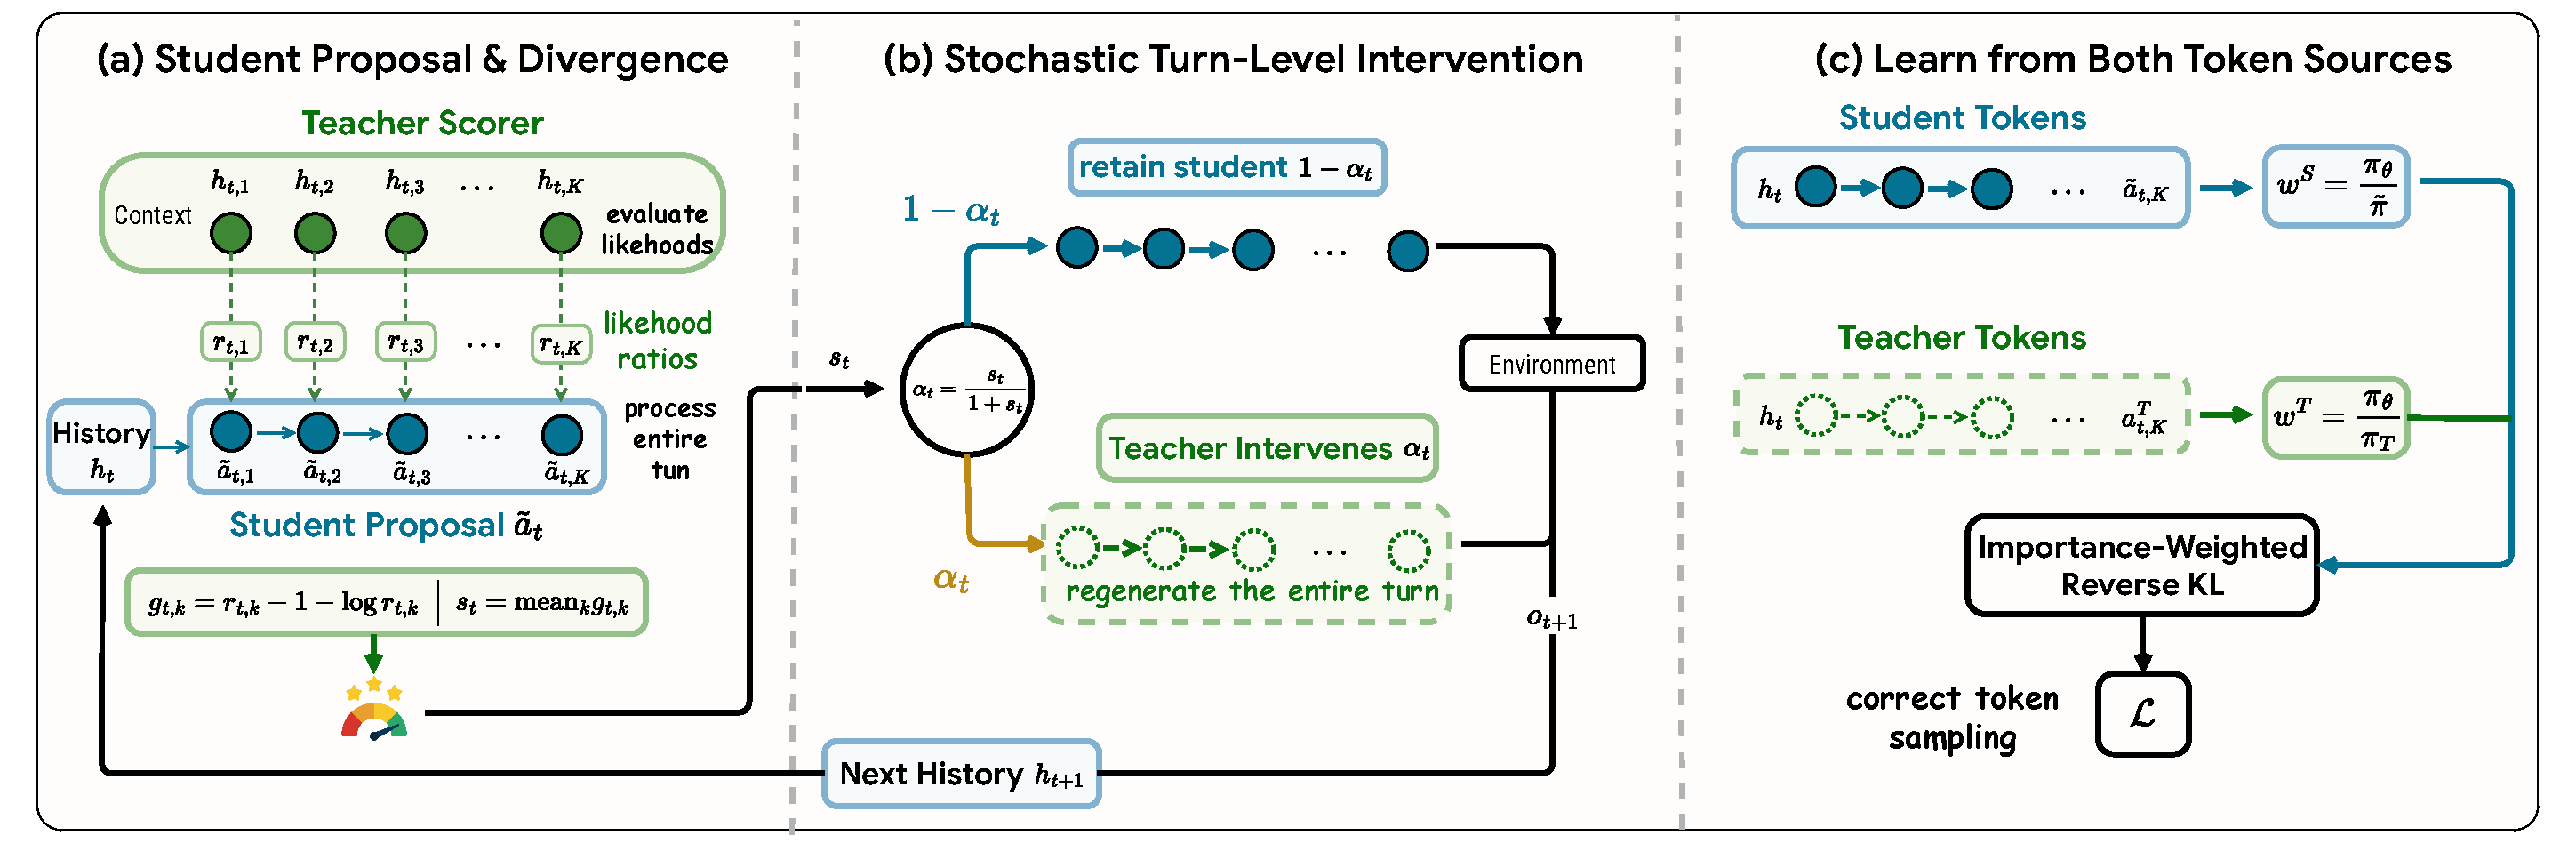
\includegraphics[width=\linewidth]{figs/frameworkv2.pdf}
    \caption{Overview of \name. A non-negative $k_3$ discrepancy estimate determines whether to retain the student proposal or replace it with a teacher-generated response before execution. The executed response is used for training, with importance ratios recovering the conditional reverse-KL expectation for teacher-generated tokens.}
    \label{fig:framework_overview}
    \vspace{-2.0em}
\end{figure}

\vspace{-0.5em}
\paragraph{On-Policy Distillation.}
Let $\pi_T$ be a fixed teacher policy and $\pi_\theta$ the trainable student policy.
In OPD, the teacher provides token-level supervision on trajectories generated by the student.
Compared with offline distillation from fixed expert trajectories, OPD reduces the mismatch between training contexts and those encountered by the student at inference time~\citep{AgarwalVZSGGB24,Gu0WH24,lu2025onpolicydistillation}.
Using reverse KL divergence, the ideal multi-turn OPD objective is
\begin{equation}
    \setlength\abovedisplayskip{1.3pt}
    \setlength\belowdisplayskip{1.3pt}
    \mathcal{L}_{\mathrm{OPD}}(\theta)
    =
    \mathbb{E}_{q\sim\mathcal{D},\,\tau\sim p_{\pi_\theta}(\cdot\mid q)}
    \left[
        \sum_{t=1}^{H}\sum_{k=1}^{L_t}
        D_{\mathrm{KL}}\!\left(
            \pi_\theta(\cdot\mid c_{t,k})
            \,\|\,
            \pi_T(\cdot\mid c_{t,k})
        \right)
    \right].
    \label{eq:multi_turn_opd}
\end{equation}
With a fixed context $c$, to reduce the heavy overhead of computing the full KL divergence, each reverse-KL term can adopt a sampling form $\mathbb{E}_{x\sim\pi_\theta(\cdot\mid c)} \left[ 
    \log\pi_\theta(x\mid c)
    -
    \log\pi_T(x\mid c)
\right]$.
Sampled OPD therefore relies on both student-induced contexts and student-generated tokens.

\vspace{-0.5em}
\paragraph{Policy Discrepancy along Trajectories.}
As discussed in \Cref{sec:introduction}, multi-turn interaction can drive the student toward histories rarely encountered under teacher rollouts, where teacher guidance may become less reliable.
Large policy discrepancies at these histories can hinder effective distillation~\citep{abs-2604-13016}.
We quantify the teacher--student policy discrepancy at history $h_t$ by
\begin{equation}
    \setlength\abovedisplayskip{1.3pt}
    \setlength\belowdisplayskip{1.3pt}
    \kappa(h_t)
    =
    D_{\mathrm{KL}}\!\left(
        \pi_\theta(\cdot\mid h_t)
        \,\|\,
        \pi_T(\cdot\mid h_t)
    \right),
    \label{eq:instantaneous_kl}
\end{equation}
where each policy defines a distribution over complete turn-level responses.
Because student actions shape subsequent observations, a deviation at one turn can affect all later decisions.
The resulting distribution shift may compound across turns and further increase policy discrepancy~\citep{abs-2604-24005,abs-2606-15912}.
This motivates intervening before a proposed response is executed, allowing teacher guidance to influence the next environment transition rather than only the training loss.


\subsection{Stochastic Teacher Intervention}
\label{sec:stochastic_teacher_intervention}

An effective intervention strategy should respond to the policy discrepancy at the current turn while accounting for uncertainty in its estimate.
Predefined schedules overlook immediate changes in discrepancy, while hard thresholds can turn estimation errors into abrupt changes in teacher control~\citep{abs-2606-15912,abs-2604-24005}.
Poor intervention decisions may therefore allow trajectory drift to persist or introduce unnecessary teacher intervention.
These considerations motivate combining an unbiased and low-variance discrepancy estimate with an intervention probability that varies smoothly with the estimated score.

 \vspace{-0.5em}
\paragraph{Turn-Level Teacher Intervention.}
We first specify how intervention modifies a rollout.
Let $\pi_{\bar\theta}$ denote the rollout student, which may be a lagged copy of the trainable policy $\pi_\theta$.
In the strictly on-policy setting, $\pi_{\bar\theta}=\pi_\theta$.
At turn $t$, the rollout student first proposes a complete response $\widetilde{a}_t\sim\pi_{\bar\theta}(\cdot\mid h_t)$.
An indicator $z_t\in\{0,1\}$ determines whether to retain this proposal ($z_t=0$) or replace it with a teacher response $a_t^T\sim\pi_T(\cdot\mid h_t)$ generated from the same history ($z_t=1$).
The resulting trajectory is
\begin{equation}
    \setlength\abovedisplayskip{1.3pt}
    \setlength\belowdisplayskip{1.3pt}
    \tau=(q,o_1,a_1,\ldots,o_H,a_H),
    \qquad
    a_t=
    \begin{cases}
        \widetilde{a}_t, & z_t=0,\\
        a_t^T, & z_t=1.
    \end{cases}
    \label{eq:intervened_trajectory}
\end{equation}
Each intervention replaces the entire response, keeping its reasoning and selected operation consistent.
For a tool call or environment action, the environment executes the operation specified in $a_t$ and returns $o_{t+1}\sim P(\cdot\mid h_t,a_t)$.
If the episode continues, the student resumes generation from $h_{t+1}=(h_t,a_t,o_{t+1})$.
Thus, $h_t$ consists of previously executed responses from either the student or the teacher, together with the corresponding environment observations.
Both policies condition on this same history at the current turn.
A discarded student proposal is neither appended to the history nor included in the training buffer.

An optimal intervention strategy must balance teacher guidance with autonomous student execution.
Unlike random intervention with predefined probabilities~\citep{abs-2606-15912} or switching at fixed thresholds, we propose a discrepancy-conditioned \emph{stochastic intervention strategy}.
The intervention probability varies smoothly with the estimated teacher--student discrepancy, allowing teacher guidance to adapt at each turn while preserving opportunities for student execution (\Cref{fig:framework_overview}~(b)).


\vspace{-0.5em}
\paragraph{Discrepancy Estimation.}
Following the policy discrepancy defined in \Cref{eq:instantaneous_kl}, we assess the current student proposal $\widetilde{a}_t=(\widetilde{x}_{t,1},\ldots,\widetilde{x}_{t,\widetilde{L}_t})$ using token-level reverse KL.
At each token position $k$, we measure the discrepancy between the student's and teacher's next-token distributions conditioned on $\widetilde{c}_{t,k}=(h_t,\widetilde{x}_{t,<k})$ using
$D_{\mathrm{KL}}(\pi_{\bar\theta}(\cdot\mid\widetilde{c}_{t,k})\|\pi_T(\cdot\mid\widetilde{c}_{t,k}))$. 

Exact evaluation requires summing over the full vocabulary at every position.
For efficiency, the common practice is to use the KL estimator~\citep{Schulman2020KL}, which requires only the teacher and student probabilities of each sampled token $\widetilde{x}_{t,k}$.
We define the teacher-to-student likelihood ratio as
\begin{equation}
    \setlength\abovedisplayskip{1.3pt}
    \setlength\belowdisplayskip{1.3pt}
    r_{t,k}
    =
    \frac{\pi_T(\widetilde{x}_{t,k}\mid\widetilde{c}_{t,k})}
         {\pi_{\bar\theta}(\widetilde{x}_{t,k}\mid\widetilde{c}_{t,k})}.
    \label{eq:teacher_student_ratio}
\end{equation} 
To provide an unbiased and low-variance estimate of the token-level reverse KL, we use the $k_3$ estimator~\citep{Schulman2020KL},
\begin{equation}
    \setlength\abovedisplayskip{1.3pt}
    \setlength\belowdisplayskip{1.3pt}
    g_{t,k}=r_{t,k}-1-\log r_{t,k}.
    \label{eq:k3_estimator}
\end{equation}
For $r_{t,k}>0$, $g_{t,k}$ is non-negative because $\log r_{t,k}\leq r_{t,k}-1$. 
Under common support, $g_{t,k}$ is a pointwise non-negative and unbiased
estimator of the token-level reverse KL under student sampling.
Moreover, in the near-policy regime, $k_3$ removes the first-order fluctuation present in $k_1$, yielding lower-order variance, which makes it a more stable signal for intervention.
We aggregate the token-level estimates into the length-normalized turn score to remove the direct scaling of the score with response length.
\begin{equation}
    \setlength\abovedisplayskip{1.3pt}
    \setlength\belowdisplayskip{1.3pt}
    s_t
    =
    \frac{1}{\widetilde{L}_t}
    \sum_{k=1}^{\widetilde{L}_t}g_{t,k}.
    \label{eq:normalized_turn_score}
\end{equation}
The score $s_t$ summarizes token-level discrepancy along the sampled proposal and serves as a length-normalized proxy for turn-level policy discrepancy.
It is distinct from the full response-level KL $\kappa(h_t)$ in \Cref{eq:instantaneous_kl}.


\vspace{-0.5em}
\paragraph{Discrepancy-Conditioned Intervention.}
To make intervention responsive to discrepancy without imposing a hard decision boundary, we set the intervention odds equal to $s_t$. 
In this paper, we adopt the following simple monotone mapping:
\begin{equation}
    \setlength\abovedisplayskip{1.3pt}
    \setlength\belowdisplayskip{1.3pt}
    \alpha_t=\frac{s_t}{1+s_t},
    \qquad
    z_t\sim\operatorname{Bernoulli}(\alpha_t),
    \label{eq:intervention_probability}
\end{equation}
where $z_t=1$ denotes teacher intervention.
This mapping assigns higher intervention probabilities to turns with larger estimated discrepancies, without a hand-tuned threshold.
When the teacher and student policies are close, the $k_3$-based score is second order in the likelihood-ratio deviation, so $\alpha_t$ remains close to zero to allow student execution and exploration.
When the policies diverge, $\alpha_t$ approaches one, increasing the likelihood of teacher intervention to correct the student's trajectory but still allowing  nonzero student execution probability with the stochastic Bernoulli sampling.


\subsection{Learning from Teacher Intervention}
\label{sec:learning_from_teacher_intervention}

Teacher intervention helps reduce error propagation across turns, but it produces mixed-policy trajectories in which executed responses may come from either the student or the teacher.
Standard OPD assumes student-generated trajectories, with the sampled reverse-KL loss taking an expectation over tokens drawn from $\pi_\theta(\cdot\mid c)$.
In intervened turns, however, the executed tokens are drawn from $\pi_T(\cdot\mid c)$.
Directly applying this loss to teacher-generated tokens without correction does not estimate the intended conditional reverse KL.
We therefore use importance-weighted reverse KL to correct this token-sampling mismatch and recover the expectation under the student policy (\Cref{fig:framework_overview}~(c)).

\vspace{-0.5em}
\paragraph{Importance-Weighted Reverse KL.}
For a teacher-generated token, we define the importance ratio as
\begin{equation}
    \setlength\abovedisplayskip{0.0pt}
    \setlength\belowdisplayskip{0.0pt}
    w_\theta(x,c)
    =
    \frac{\pi_\theta(x\mid c)}{\pi_T(x\mid c)}.
    \label{eq:teacher_importance_ratio}
\end{equation}
Assuming that $\pi_\theta(\cdot\mid c)$ is absolutely continuous with respect to $\pi_T(\cdot\mid c)$, importance sampling yields
\begin{equation}
    \setlength\abovedisplayskip{1.3pt}
    \setlength\belowdisplayskip{1.3pt}
\begin{split}
    &\mathbb{E}_{x\sim\pi_T(\cdot\mid c)}
    \left[
        w_\theta(x,c)
        \log\frac{\pi_\theta(x\mid c)}{\pi_T(x\mid c)}
    \right] =
    \sum_x \pi_T(x\mid c)
    \frac{\pi_\theta(x\mid c)}{\pi_T(x\mid c)}
    \log\frac{\pi_\theta(x\mid c)}{\pi_T(x\mid c)} \\
    &\quad=
    \mathbb{E}_{x\sim\pi_\theta(\cdot\mid c)}
    \left[
        \log\frac{\pi_\theta(x\mid c)}{\pi_T(x\mid c)}
    \right]
    =
    D_{\mathrm{KL}}\!\left(
        \pi_\theta(\cdot\mid c)
        \,\|\,
        \pi_T(\cdot\mid c)
    \right).
\end{split}
    \label{eq:importance_weighted_reverse_kl}
\end{equation}
Teacher-generated tokens can therefore estimate the same conditional reverse-KL term once their token-sampling distribution is corrected.


\vspace{-0.5em}
\paragraph{Combined Training Objective.}
Once the task is complete, the full executed trajectory is added to the training buffer.
Consequently, each turn contributes either the retained student proposal when $z_t=0$ or the regenerated teacher response when $z_t=1$.
For a retained student token, no sampling correction is required because
$\widetilde{x}_{t,k}$ is already sampled from $\pi_\theta$.
For a teacher-generated token, we define the importance ratio as $\omega^{T}_{t,k}(\theta) = \pi_\theta(x^{T}_{t,k}\mid c^{T}_{t,k}) /\pi_T(x^{T}_{t,k}\mid c^{T}_{t,k})$.
Following the standard OPD formulation based on sampled tokens, the optimization objective is the empirical mean of the sampled reverse-KL terms over all generated tokens:
\begin{equation}
    \setlength\abovedisplayskip{1.3pt}
    \setlength\belowdisplayskip{1.3pt}
    \widehat{\mathcal{L}}_{\name}(\theta)
    =
    \frac{1}{N_{\mathrm{tok}}}
    \sum_{t=1}^{H}
    \left[
        (1-z_t)
        \sum_{k=1}^{\widetilde{L}_t}
        \ell_\theta(
            \widetilde{x}_{t,k},
            \widetilde{c}_{t,k}
        )
        +
        z_t
        \sum_{k=1}^{L_t^T}
        \omega^T_{t,k}(\theta)
        \ell_\theta(
            x^T_{t,k},
            c^T_{t,k}
        )
    \right],
    \label{eq:intervention_corrected_objective}
\end{equation}
where $\ell_\theta(x,c)=\log\pi_\theta(x\mid c)-\log\pi_T(x\mid c)$ is the token-level student-to-teacher log-ratio, whose expectation under $x\sim\pi_\theta(\cdot\mid c)$ equals the conditional reverse KL, and $N_{\mathrm{tok}}=\sum_{t=1}^{H}((1-z_t)\widetilde{L}_t+z_tL_t^T)$ is the number of optimization tokens in the episode.  
For retained student turns, the first term is exactly the standard sampled OPD objective because the tokens are drawn from $\pi_\theta$.
For intervened turns, the second term uses importance weighting to correct the change in token-sampling distribution from $\pi_T$ to $\pi_\theta$.
By \Cref{eq:importance_weighted_reverse_kl}, both branches therefore estimate the same conditional reverse-KL objective at their respective sampled contexts. 
Importantly, the identity in \Cref{eq:importance_weighted_reverse_kl} holds at a fixed context.
The importance correction accounts for the token-sampling distribution of the teacher branch, but does not undo the adaptive intervention decision or correct the distribution over contexts induced by intervention, including teacher-generated prefixes and subsequent interaction histories.



